\documentclass[11pt,letterpaper]{article}
\usepackage[margin=1in]{geometry}
\usepackage{graphicx} % Required for inserting images
\usepackage{tikz}
\usepackage{amsthm,amsmath,amssymb}
\usepackage{algorithm}
\usepackage{algpseudocode}
\usepackage{xcolor}
\usepackage{soul}
\usepackage{enumitem}

\usepackage[hidelinks]{hyperref}
\usepackage{cleveref}

% Theorems
\newtheorem{theorem}{Theorem}[section]
\newtheorem{corollary}[theorem]{Corollary}
\newtheorem{lemma}[theorem]{Lemma}
\newtheorem{claim}[theorem]{Claim}
\theoremstyle{definition}
\newtheorem{definition}[theorem]{Definition}
\newtheorem{remark}[theorem]{Remark}
\newtheorem{observation}[theorem]{Observation}

\crefname{theorem}{Theorem}{Theorems}
\Crefname{theorem}{Theorem}{Theorems}
\crefname{corollary}{Corollary}{Corollaries}
\Crefname{corollary}{Corollary}{Corollaries}
\crefname{lemma}{Lemma}{Lemmas}
\Crefname{lemma}{Lemma}{Lemmas}
\crefname{claim}{Claim}{Claims}
\Crefname{claim}{Claim}{Claims}
\crefname{definition}{Definition}{Definitions}
\Crefname{definition}{Definition}{Definitions}
\crefname{remark}{Remark}{Remarks}
\Crefname{remark}{Remark}{Remarks}
\crefname{observation}{Observation}{Observations}
\Crefname{observation}{Observation}{Observations}

\newcommand{\reals}{\mathbb{R}}
\newcommand{\Span}{\mathrm{span}}
\newcommand{\coreq}{\mathrm{coreq}}

\newcommand{\calA}{\mathcal{A}}
\newcommand{\calB}{\mathcal{B}}
\newcommand{\calC}{\mathcal{C}}
\newcommand{\calD}{\mathcal{D}}
\newcommand{\calE}{\mathcal{E}}
\newcommand{\calF}{\mathcal{F}}
\newcommand{\calG}{\mathcal{G}}
\newcommand{\calH}{\mathcal{H}}
\newcommand{\calI}{\mathcal{I}}
\newcommand{\calJ}{\mathcal{J}}
\newcommand{\calK}{\mathcal{K}}
\newcommand{\calL}{\mathcal{L}}
\newcommand{\calM}{\mathcal{M}}
\newcommand{\calN}{\mathcal{N}}
\newcommand{\calO}{\mathcal{O}}
\newcommand{\calP}{\mathcal{P}}
\newcommand{\calQ}{\mathcal{Q}}
\newcommand{\calR}{\mathcal{R}}
\newcommand{\calS}{\mathcal{S}}
\newcommand{\calT}{\mathcal{T}}
\newcommand{\calU}{\mathcal{U}}
\newcommand{\calV}{\mathcal{V}}
\newcommand{\calW}{\mathcal{W}}
\newcommand{\calX}{\mathcal{X}}
\newcommand{\calY}{\mathcal{Y}}
\newcommand{\calZ}{\mathcal{Z}}

\newcommand{\cost}{\mathrm{COST}}
\newcommand{\ALG}{\mathrm{ALG}}
\newcommand{\OPT}{\mathrm{OPT}}
\newcommand{\Flow}{\textsc{Flow}}
\newcommand{\ouralg}{\textsc{LineTracker}}

\newcommand{\EE}{\mathbb{E}}

\newcommand{\interval}[1]{\lfloor #1 \rceil}
\newcommand{\dis}[1]{#1}
\newcommand{\off}{\mathrm{off}}
\newcommand{\on}{\mathrm{on}}
\newcommand{\org}{\mathrm{org}}
\newcommand{\rel}{\mathrm{rel}}
\newcommand{\new}{\mathrm{new}}

\newcommand{\solution}{\medskip\noindent\textbf{Solution.}\par\medskip}

\title{21-701: Discrete Mathematics \\ Homework 1}
\author{Poon Tze-Yang}
\date{Due September 9, 2026}


\begin{document}

\maketitle

\noindent Instructor: Wesley Pegden

\begin{enumerate}
\item In class we used the probabilistic method to prove that $m(k) \geq 2^{k-1}$, where $m(k)$ is the fewest number of edges in any $k$-uniform hypergraph that is not 2-colorable. Now define $m(k;n)$ to be the fewest number of edges in any $k$-uniform hypergraph on $n$ vertices that is not 2-colorable.
\begin{enumerate}
\item By tweaking the probabilistic proof we gave, prove that
\[
m(k;2n) \geq \frac{\binom{2n}{n}}{2\binom{2n-k}{n}}.
\]
\item Prove that for every $n \geq k \geq 1$, this bound is stronger than the $2^{k-1}$ bound on $m(k)$, but that for any fixed $k$ the limit of this bound as $n \to \infty$ is $2^{k-1}$.
\item \textbf{Extra, not to be handed in:} Prove a similar bound on $m(k;2n+1)$ and use these bounds to upgrade our result $m(k) \geq 2^{k-1}$ from class to the bound $m(k) > 2^{k-1}$. In particular, we learn that graphs with only 2 edges are 2-colorable $\smile$.
\end{enumerate}
\end{enumerate}

\solution
\paragraph{(a)} 
Let $\ell = \frac{\binom{2n}{n}}{2\binom{2n-k}{n}}$ Let $\calH$ be a $k$-uniform hypergraph on $2n$ vertices with $<\ell$ edges. 
There are $\binom{2n}{n}$ colorings which color $n$ vertices red and $n$ vertices blue.
We select one of these colorings uniformly at random.
For each edge $f$, of the above colorings, there are $2\binom{2n-k}{n}$ of them in which $f$ is monochromatic (there are two possible monochromtic colorings of $f$, and for each monochromatic coloring there are $\binom{2n-k}{n}$ ways to color the remaining vertices).
Let $\varepsilon_f$ be the event that $f$ is monochromatic. We have
\begin{align*}
    \Pr(\varepsilon_f) = \frac{2\binom{2n-k}{n}}{\binom{2n}{n}}.
\end{align*}
By the union bound, the probability that any of the $\ell$ edges is monochromatic is
\begin{align*}
    \Pr\left(\bigcup_{f\in\calH}\varepsilon_f\right) \leq \sum_{f\in \calH} \Pr\left(\varepsilon_f\right) = \ell  \Pr(\varepsilon_f)<1.
\end{align*} 
Hence, there must exist a 2-coloring of $\calH$.

\paragraph{(b)}
The bound is tighter:
\begin{align*}
    \frac{\binom{2n}{n}}{2\binom{2n-k}{n}} = \frac{\prod_{i=2n-k+1}^{2n}i}{2\prod_{i=n-k+1}^{n}i} = \frac{1}{2}\prod_{i=1}^{k}\frac{2n-k+i}{n-k+i}<\frac{1}{2}\cdot 2^k = \frac{1}{2^{k-1}}.
\end{align*}
We have that 
\begin{align*}
    \lim_{n\to \infty}\frac{2n-k+i}{n-k+i} = 2 + \lim_{n\to\infty}\frac{k-i}{n-k+i} = 2.
\end{align*}
So 
\begin{align*}
    \lim_{n\to\infty}\frac{\binom{2n}{n}}{2\binom{2n-k}{n}} = \frac{1}{2}\lim_{n\to\infty} \prod_{i=1}^{k}\frac{2n-k+i}{n-k+i} = 2^{k-1}.
\end{align*}

\begin{enumerate}[resume]
\item Recall that $m(k)$ is the least $m$ such that there is a $k$-uniform hypergraph on $m$ edges that is not 2-colorable. Prove that $m(k) = O(k^2 2^k)$.

\emph{Hint:} Generate a $k$-uniform hypergraph by choosing $m$ edges randomly and independently.
\end{enumerate}

\solution

We construct a $k$-uniform hypergraph $\calH$ on $k^2$ vertices by (at most) $m$ edges independently at random.
Concretely, for $i$ in $[m]$, we sample hyperedge $f_i$ uniformly at random among all $k$-hyperedges, and define $\calH := \bigcup_{i\in[m]}f_i$.
Let $\calA$ be the event that $\calH$ is 2-colorable. 
For a 2-coloring $C$ of $\calH$, let $\calB_C$ be the event that $C$ is proper.
For a given hyperedge $f_i$, let $\calC_{C,f_i}$ be the event that the edge $f_i$ is not monochromatic in $C$.

First, we consider the probability that each 2-coloring is proper. By the independence of selecting each edge, 
    \begin{align*}
        \Pr(\calB_C) = \Pr\left(\bigcap_{i\in [m]}\calC_{C,f_i}\right) = \prod_{i\in [m]}\Pr\left(\calC_{C,f_i}\right).
    \end{align*}
    Let coloring $C$ assign $a$ vertices to one color and $b$ vertices to the other, so $a+b = k^2$. 
    For each hyperedge $f_i$,
    \begin{align*}
        \Pr(\calC_{C,f_i}) &= 1 - \Pr(f_i\text{ is monochromatic in }C) \\
        & = 1- \frac{\# k\text{-hyperedges on vertices in first color} + \# k\text{-hyperedges on vertices in second color}}{\# k\text{-hyperedges on }k^2\text{ vertices}} \\
        & = 1- \frac{\binom{a}{k} + \binom{b}{k}}{\binom{k^2}{k}} \\
        & \leq 1 - 2\cdot \frac{\binom{\frac{k^2}{2}}{k}}{\binom{k^2}{k}} \qquad \qquad(\binom{x}{k}\text{ is convex in }x)
    \end{align*}
Let $\ell = \frac{\binom{\frac{k^2}{2}}{k}}{\binom{k^2}{k}}$. Then we have $\Pr(\calB_C) \leq (1-2\ell)^m$.

By the union bound,
\begin{align*}
    \Pr(\calA) &= \Pr\left(\bigcup_{C \text{ is a coloring}}\calB_C\right) \\
    &= \sum_{C \text{ is a coloring}}\Pr\left(\calB_C\right)\leq 2^{k^2}\left(1-2\ell\right)^m \\
    &= \exp\left(k^2\ln 2 + m\ln(1-2\ell)\right).
\end{align*}

So $\Pr(\calA)<1$ if $k^2\ln 2 + m\ln(1-2\ell)<0$, which is equivalent to $m > \frac{k^2\ln 2}{-\ln(1-2\ell)}$.
By the Taylor's series for $\ln(1-x)\approx -x$, it suffices to choose $m = O(\frac{k^2}{\ell})$
Expanding $\ell$:
\begin{align*}
    \ell = \frac{\binom{\frac{k^2}{2}}{k}}{\binom{k^2}{k}} &=\prod_{i=0}^{k-1}\frac{\frac{k^2}{2}-i}{k-i}=2^{-k}\prod_{i=0}^{k-1}\frac{k^2-2i}{k^2-i}.
\end{align*}
The additional product term is small, so $m=O(k^2 2^k)$ suffices.

\begin{enumerate}[resume]
\item Say a \emph{leveled hypergraph} is a collection of leveled edges $f\subseteq V$ partitioned into pairs $(f^+,f^-)$, $f = f^+\mathbin{\dot{\cup}}f^-$ consisting of the \emph{top} ($f^+$) and the \emph{bottom} ($f^-$). (Because of the next definition we are only interested in the case where $f^+$ and $f^-$ are both nonempty for every edge.)

We say a leveled hypergraph is \emph{upside-down} if for all distinct leveled edges $f,g\in\calH$, the top of $f$ intersects the bottom of $g$ (and vice versa).

Give a probabilistic proof that for an upside-down leveled hypergraph, we have
\[
\sum_{f\in\calH}\frac{1}{\binom{|f|}{|f^+|}} \leq 1.
\]

\emph{Hint:} Start by defining a leveled hypergraph $\calF$ with as many leveled edges as you can muster that has the property that any upside-down hypergraph shares at most one leveled edge with $\calF$.
\end{enumerate}

\solution

Order the vertices of $V = \{v_1,.., v_n\}$.
Let $\calF$ be the leveled hypergraph with one edge $f$ for each subset of $U\subseteq V$ and each $i\in \{1,..,|U|-1\}$. 
The vertices of $f$ are exactly $U$ and the bottom $f^-$ are the first $i$ vertices of $U$ in the ordering above.

\begin{lemma} \label[lemma]{lemma:intersectionAtMostOne}
    Each upside-down hypergraph shares at most one leveled edge with $\calF$.
\end{lemma}
\begin{proof}
    For any two hyperedges $f,h\in \calF$ such that $h\in \calH$. Let $u$ (resp. $v$) be the largest vertex in $f^-$ (resp. $h^-$), according to the order above.
    If $u\geq v$, then $f^+\cap h^-= \emptyset$. Similarly,  if $u< v$, then $f^-\cap h^+ = \emptyset$.
    Thus, $f\notin \calF$.
\end{proof}

\begin{lemma} \label[lemma]{lemma:correctNumberOfEdges}
    For integers $0<k<\ell \leq n$, the number of edges in $\calF$ with $\ell$ vertices and $k$ top vertices is $\binom{n}{\ell}$.
\end{lemma}
\begin{proof}
    Each subset $U\subseteq V$ of size $\ell$ is in bijection with the edge $f\in \calF$ of size $\ell$ with its last $k$ elements in $f^+$. 
\end{proof}

Let $\pi$ by a uniformly random permutation of the vertices.
For $h\in \calH$, let $\xi_{h}$ be the indicator event that $h=\pi f$.
By linearity of expectation on the expected number of intersections and \cref{lemma:intersectionAtMostOne}, 
\begin{align*}
    \sum_{h\in \calH}\EE[\xi_h]= \EE\left[\sum_{h\in \calH}\xi_h\right] \leq 1.
\end{align*}

For each individual $h\in \calH$, by \cref{lemma:correctNumberOfEdges} we have 
\begin{align*}
    \EE[\xi_h] &= \sum_{f\in \calF}\Pr(h = \pi f) \\
    &= \sum_{\substack{f\in \calF \text{ s.t.} \\ |f| = |h| \text{ and } |f^+| = |h^+|}} \frac{1}{\binom{n}{|f|}}\cdot \frac{1}{\binom{|f|}{|f^+|}} \\
    &= \frac{1}{\binom{|h|}{|h^+|}}.
\end{align*}

Thus,
\begin{align*}
    \sum_{h\in\calH}\frac{1}{\binom{|h|}{|h^+|}} \leq 1.
\end{align*}

\begin{enumerate}[resume]
\item A \emph{dominating set} of a graph $G$ is a set $U\subseteq V(G)$ with the property that every vertex of $G$ either lies in $U$ or is adjacent to a vertex of $U$. Prove that every graph $G$ on $n$ vertices with minimum degree $\delta\geq 1$ has a dominating set of size at most
\[
n\cdot\frac{1+\ln(\delta+1)}{\delta+1}.
\]

\emph{Hint:} alterations
\end{enumerate}

\solution

We first include each vertex with probability $p$, independently.
Let $X$ be the random variable for the number of vertices selected this way, so $\EE[X] = np$.
Let $Y$ be the random variable for the number of vertices which are not selected and all their neighbors are not selected.
Then by linearity of expectation, $\EE[Y] \leq n(1-p)^{\delta+1}$, and if we select all $X+Y$ vertices we get a dominating set.
We get
\begin{align*}
    \EE[X+Y] = pn + (1-p)^{\delta+1}n.
\end{align*}
This is minimized at 
\begin{align*}
    p = 1 - \left(\frac{1}{\delta+1}\right)^\frac{1}{\delta}.
\end{align*}
Then we have 
\begin{align*}
    \EE[X+Y]&= n\left(1-\left(\frac{1}{\delta+1}\right)^\frac{1}{\delta} + \left(\frac{1}{\delta+1}\right)^\frac{\delta+1}{\delta}\right)\\
    &= n\left(\frac{1+\delta - (\delta+1)\left(\frac{1}{\delta+1}\right)^\frac{1}{\delta} + \left(\frac{1}{\delta+1}\right)^\frac{1}{\delta}}{\delta+1}\right)\\
    &= n\left(\frac{1+\delta\left(1-\left(\frac{1}{\delta+1}\right)^\frac{1}{\delta}\right)}{\delta+1}\right) \\
    &= n\left(\frac{1+\delta\left(1-e^{\frac{1}{\delta}\ln(\delta+1)}\right)}{\delta+1}\right) \\
    &\leq n\left(\frac{1+\ln(\delta+1)}{\delta+1}\right).
\end{align*}
So there is at least one dominating set of sufficiently small size.

\noindent In class we briefly discussed an explicit construction that gives triangle-free graphs of arbitrarily large chromatic number. Here is another one:

\begin{enumerate}[resume]
\item Define the operation $M(G)$ on a graph $G$ via the following procedure:
\begin{enumerate}[label=(\roman*)]
\item For each $v\in G$, add a paired vertex $\bar{v}$.
\item Create a single new vertex $x_0$.
\item The edges of $M(G)$ are all the edges of $G$, together with all edges of the form $\{v,\bar{u}\}$ where $v$ is adjacent to $u$, and all edges of the form $\{\bar{v},x_0\}$, for all $v\in G$.
\end{enumerate}

Here is an example of $M(G)$ when the graph $G$ is a 5-cycle:
\begin{center}
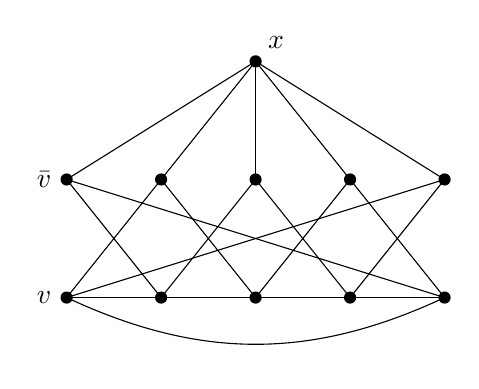
\begin{tikzpicture}[scale=1, line width=0.4pt]
\foreach \i in {0,...,4} {
    \coordinate (v\i) at (\i*1.2, 0);
    \coordinate (u\i) at (\i*1.2, 1.5);
}
\coordinate (x) at (2.4, 3);

% edges of G among the v_i (a 5-cycle)
\draw (v0) -- (v1) -- (v2) -- (v3) -- (v4);
\draw (v4) to[bend left=25] (v0);

% edges {v_i, \bar u} where v_i is adjacent to u in G
\foreach \i in {0,...,4} {
    \pgfmathtruncatemacro{\ip}{mod(\i+1,5)}
    \pgfmathtruncatemacro{\im}{mod(\i+4,5)}
    \draw (v\i) -- (u\ip);
    \draw (v\i) -- (u\im);
}

% edges {\bar v_i, x_0}
\foreach \i in {0,...,4} {
    \draw (u\i) -- (x);
}

\foreach \i in {0,...,4} {
    \fill (v\i) circle (2.2pt);
    \fill (u\i) circle (2.2pt);
}
\fill (x) circle (2.2pt);

\node[left=2pt] at (v0) {$v$};
\node[left=2pt] at (u0) {$\bar v$};
\node[above right=1pt] at (x) {$x$};
\end{tikzpicture}
\end{center}

Note that if $G$ is triangle-free then so is $M(G)$. Prove that if $G$ has chromatic number $k$ then $M(G)$ has chromatic number $k+1$, and moreover if $G$ is $k$-critical ($G$ has chromatic number $k$ but every proper subgraph is $(k-1)$-colorable) then $M(G)$ is $(k+1)$-critical.
\end{enumerate}

\solution

Partition the vertices of $M(G)$ into $V\cup \bar{V} \cup\{x\}$.
 
\paragraph{$M(G)$ is $(k+1)$-colorable.}
Color all vertices in $V$ and $\bar{V}$ with their corresponding color in $G$.
Color $x$ with the new color. 
Each of vertices $u\in V\cup \bar{V}$ is incident only to vertices $v$ or $\bar{v}$ in pairs $(v,\bar{v})$ corresponding to vertices $v$ in $G$ which $u$ are adjacent to.
Hence, by the $k$-colorability of $G$, this is a valid coloring.

\paragraph{$M(G)$ is not $k$-colorable.}

Suppose $M(G)$ was $k$-colorable. Let $x$ be colored $c_1$.
Then, none of the vertices $\bar{V}$ are colored $c_1$. 
If we can obtain a coloring that recolors all $c_1$-colored vertices in $V$, we have obtained $(k-1)$-coloring of $G$, which is a contradiction.

First, consider all pairs $(v,\bar{v})$ which are differently-colored and $v$ is not colored $c_1$. 
Let $v$ be colored $c_2$.
Note that $\bar{v}$'s color can be changed to $c_2$, since all vertices adjacent to $\bar{v}$ are adjacent to $v$, except $x$, which is not colored $c_2$.

Now, consider the remaining pairs $(v,\bar{v})$ which are differently-colored.
Vertices $v$ must be colored $c_1$, and consider a single pair where $\bar{v}$ is colored $c_3$.
We will recolor each $v$ to be the same color as its $\bar{v}$.
Note that no two such pairs can have $v$'s that are adjacent to each other, since both $v$'s start out with color $c_1$.
Therefore, all pairs adjacent to the current $(v,\bar{v})$ pair are similarly colored, so recoloring $v$ to $c_3$ does not introduce any conflicting pairs.
This gives a contradiction to the fact that $\chi(G) = k$.

\paragraph{$M(G)$ is $(k+1)$-critical.}

It suffices to show that removing any edge from $M(G)$ results in a $k$-colorable graph.

If we remove any edge $(u,v)$ for $u,v\in V$, by the criticality of $G$, we can recolor all vertices of $V$ with $k-1$ colors. 
Copying these colors onto the shadow vertices gives a valid $k$-coloring.

If we remove any edge $(x,\bar{v})$, first recolor all vertices of $V-v$ with $k-1$ colors.
Copy these colors onto $\bar{V} - \bar{v}$. 
Finally, color $v,\bar{v}$ and $x$ with the $k$-th color.

Finally, if we remove any edge $(\bar{u},v)$, consider the graph $G$ with the edge $(v,u)$ removed.
By the criticality of $G$, we can recolor all vertices of $V$ with $k-1$ colors, with the only possible conflict being on the edge $(u,v)$.
Copy these colors onto $\bar{V}$, with the only possible additional conflict being on the edge $(u,\bar{v})$.
To fix this, recolor $u$ with the $k$-th color, which is the same color we use on $x$.
This gives a valid $k$-coloring of $M(G)$.

\end{document}
